\documentclass[12pt]{memoir}\usepackage[]{graphicx}\usepackage[table]{xcolor}
% maxwidth is the original width if it is less than linewidth
% otherwise use linewidth (to make sure the graphics do not exceed the margin)
\makeatletter
\def\maxwidth{ %
  \ifdim\Gin@nat@width>\linewidth
    \linewidth
  \else
    \Gin@nat@width
  \fi
}
\makeatother

\definecolor{fgcolor}{rgb}{0.345, 0.345, 0.345}
\newcommand{\hlnum}[1]{\textcolor[rgb]{0.686,0.059,0.569}{#1}}%
\newcommand{\hlstr}[1]{\textcolor[rgb]{0.192,0.494,0.8}{#1}}%
\newcommand{\hlcom}[1]{\textcolor[rgb]{0.678,0.584,0.686}{\textit{#1}}}%
\newcommand{\hlopt}[1]{\textcolor[rgb]{0,0,0}{#1}}%
\newcommand{\hlstd}[1]{\textcolor[rgb]{0.345,0.345,0.345}{#1}}%
\newcommand{\hlkwa}[1]{\textcolor[rgb]{0.161,0.373,0.58}{\textbf{#1}}}%
\newcommand{\hlkwb}[1]{\textcolor[rgb]{0.69,0.353,0.396}{#1}}%
\newcommand{\hlkwc}[1]{\textcolor[rgb]{0.333,0.667,0.333}{#1}}%
\newcommand{\hlkwd}[1]{\textcolor[rgb]{0.737,0.353,0.396}{\textbf{#1}}}%
\let\hlipl\hlkwb

\usepackage{framed}
\makeatletter
\newenvironment{kframe}{%
 \def\at@end@of@kframe{}%
 \ifinner\ifhmode%
  \def\at@end@of@kframe{\end{minipage}}%
  \begin{minipage}{\columnwidth}%
 \fi\fi%
 \def\FrameCommand##1{\hskip\@totalleftmargin \hskip-\fboxsep
 \colorbox{shadecolor}{##1}\hskip-\fboxsep
     % There is no \\@totalrightmargin, so:
     \hskip-\linewidth \hskip-\@totalleftmargin \hskip\columnwidth}%
 \MakeFramed {\advance\hsize-\width
   \@totalleftmargin\z@ \linewidth\hsize
   \@setminipage}}%
 {\par\unskip\endMakeFramed%
 \at@end@of@kframe}
\makeatother

\definecolor{shadecolor}{rgb}{.97, .97, .97}
\definecolor{messagecolor}{rgb}{0, 0, 0}
\definecolor{warningcolor}{rgb}{1, 0, 1}
\definecolor{errorcolor}{rgb}{1, 0, 0}
\newenvironment{knitrout}{}{} % an empty environment to be redefined in TeX

\usepackage{alltt}
\newcommand{\acctitle}{Math 106 Gini Index Notes}
\usepackage{latexsym, amssymb, booktabs, hyperref, amsmath, mathptmx, graphicx, framed}
\usepackage[table]{xcolor}
\usepackage[bottom]{footmisc}
\usepackage{endnotes}
\usepackage{makecell}
\let\footnote=\endnote

\OnehalfSpacing
\setaftersecskip{1sp}

\hypersetup{%
 pdftitle={\acctitle},
 pdfdisplaydoctitle=true,
 pdflang={en-US}
 }

% booktabs hack 
 \aboverulesep=0ex
 \belowrulesep=0ex
 \renewcommand{\arraystretch}{1.2}
 
\parindent = 0pt
\addtolength{\parskip}{0.5\baselineskip}
\usepackage[margin = 1.5in]{geometry}
\IfFileExists{upquote.sty}{\usepackage{upquote}}{}
\begin{document}
%\SweaveOpts{concordance=TRUE}
\title{\acctitle}

\section*{Introduction}
\bigskip

An editorial in the August 8, 2017 issue of \emph{Nature Human Behavior} states: 
\begin{quote}
Economic inequality has become a serious concern for many in the political,
public and academic spheres. The gap between rich and poor has been increasing
for decades, to the extent that more than 50\% of the world's wealth is now held
by the top 1\% of earners. The geography of inequality can be mapped against
poorer health standards, lesser educational attainment, higher crime rates,
greater unhappiness and lack of trust in one's fellow citizens.

Research in psychology and economics provides a seeming paradox when compared
with these grim statistics of growing inequality in wealth and income. Numerous
laboratory-based studies have shown that people reject unfair payment distributions.
Participants even reject inequitable outcomes on behalf of unknown others in
third-party scenarios. This work suggests that equality should be a powerful and
desirable social norm. However, if this is the case, why is wealth inequality so tolerated in
real life\footnote{Understanding attitudes to inequality. \emph{Nat Hum Behav} 1, 0166
(2017). https://doi.org/10.1038/s41562-017-0166}?
\end{quote}
There is evidence showing that it may not be so much that people \emph{tolerate} wealth 
inequality, but rather that people may not have a clear understanding of the actual distribution of wealth in 
whatever populations they belong to.  In a paper\footnote{Norton, M. I., \& Ariely, D. (2011).
Building a Better America---One Wealth Quintile at a Time. \emph{Perspectives on Psychological Science}, 6(1),
9--12. https://doi.org/10.1177/1745691610393524"} published in 2011, Michael I. Norton and Dan Ariely 
present evidence supporting this proposition. They report results of a study that shows Americans have
misconceptions about the distribution of wealth in their country.  Wealth inequality is an 
issue in many countries, but much of the research on this subject focuses on the USA.

The following three bar graphs, which appear in their paper, summarize average views
regarding the actual, perceived, and ideal distributions of wealth in the USA.

\begin{center}
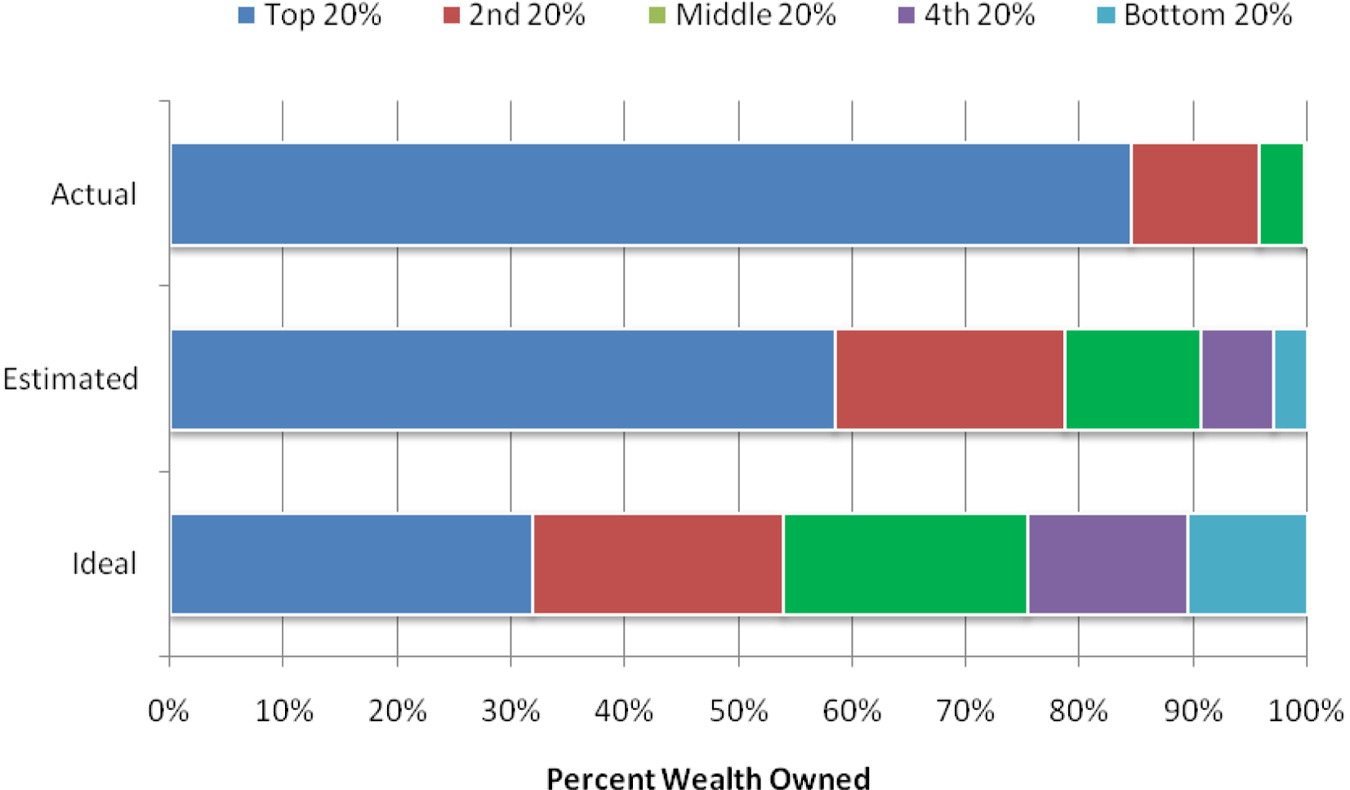
\includegraphics[width = 12cm]{graphs/bargraph.jpeg}
\end{center}

The top graph (labeled ``Actual") shows that the wealthiest one-fifth (20\%) of the US population owns
about 84\% of the wealth.  The next wealthiest fifth owns about 11\%.  The third
wealthiest own 4\% and the bottom two fifths own $0.2\%$ and $0.1\%$, respectively. 
The shares of the two bottom fifths are actually too small to be visible on the graph.

The next graph shows what Americans estimate the distribution of wealth to be,
on average, and the last one shows an ``ideal" distribution of wealth, according
to the average American.  Both of these graphs show a much more equal distribution
than the actual one. These three graphs indicate that on average, Americans
do not have an accurate understanding of the actual distribution of wealth in 
the country. 

Whatever the facts are, it's not clear that we should expect the average citizen 
to be able to cite accurate statistics on this matter, without first studying it 
carefully.  We do encounter statements of the form ``The top $x\%$ owns $y\%$ of the wealth"
frequently in various media but it can be hard to keep the numbers straight.  
Furthermore, the mathematics of the distribution of wealth is less intuitive
than one might think.  For example, roughly 10\% of American households
actually have \emph{negative} net worth, by some measures.  This means that a single 
family with a positive net worth, say US\$100, owns more wealth than the bottom 10\% of 
American families.  The purpose of this document is to help you understand some of the 
most commonly measures of wealth inequality so that you can read further on the subject.

\subsection*{A Clarification}

We will focus on \emph{wealth} inequality, as opposed to \emph{income} inequality
here.  The measures we cover will be applicable to both, as they are related 
but distinct issues that are frequently discussed together.

\section*{The Hoover Index}

% (1936) The Measurement of Industrial Localization, \emph{Review of Economics and Statistics}, 18, No. 162--71
The first measure of wealth inequality we consider is called the \emph{Hoover Index} (named after the economist
Edgar M. Hoover, Jr.), or sometimes the \emph{Robin Hood Index}.  This second name refers to the fictional hero of English legend who stole from the rich and gave to the poor.  How much (in percent terms) would Robin Hood have
to steal from the rich and give to the poor, in order that everyone ends up with the same wealth?
That's essentially what the Hoover/Robin Hood index is.  

Here's a more formal definition:  The \emph{Hoover Index} (also called \emph{Robin Hood Index} of a population is the percentage of total wealth that would have to be redistributed in order for every individual to have the same wealth.  We will call this number $H$.

\subsection*{Example 1}
We'll consider an intuitive, visual example involving a population with 20 individuals.
Here's a bar graph showing the wealth per person (each person corresponds to a single bar).
The people are sorted so that the wealth increases as we move to the right.  The blue
line indicates the mean wealth per person.


\begin{center}
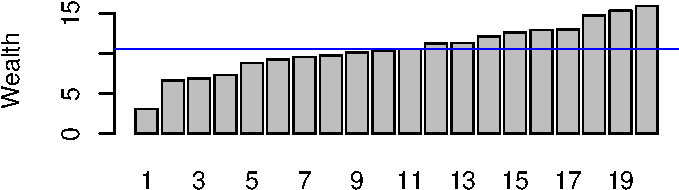
\includegraphics{figure/bar2-1.pdf}
\end{center}
You can imagine slicing the bars that extend above the blue line:

\begin{center}
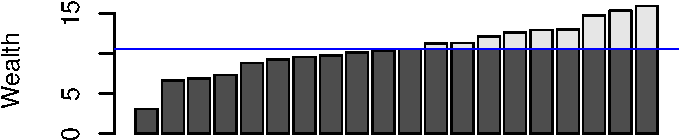
\includegraphics{figure/bar3-1.pdf}
\end{center}
Now glue these pieces to the shorter bars in such a way that every bar reaches exactly to 
the blue line:

\begin{center}
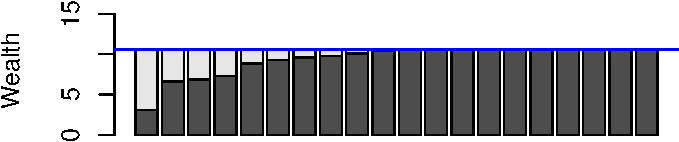
\includegraphics{figure/bar4-1.pdf}
\end{center}
In effect, this redistributes the wealth to achieve 100\%
equality. 

The Hoover Index equals the area of the bars that was sliced off, divided by the 
total area, times 100\%. In the chart above, the Hoover Index equals the 
light gray area divided by the area of the entire shaded region 
which here is approximately 11\%.  

%\subsubsection*{Example 2}  We'll first consider a very small population---only two
%people. Suppose Erin has wealth \$50{,}000 and Kelvin owns \$100{,}000.
%Find the Hoover Index for this population. 

%\begin{quote}
%\emph{Solution}: To equalize wealth among this population, we could take
%\$25{,}000 from Kelvin and give it to Erin. Then each person would have \$75{,}000.

%The total wealth in the population is $\$50{,}000 + \$100{,}000 = \$150{,}000$, 
%so the Hoover Index is: 

%$$\dfrac{\$25{,}000}{\$150{,}000}\times 100\% = 16.7.\%$$

%\emph{Comments}: How do I know there aren't other ways to equalize the 
%wealth of Erin and Kelvin by transferring different amounts of money, which 
%could result in a different Hoover Index?  We have defined this new quantity 
%$H$, and at some point we should verify that for a given population and 
%distribution of wealth, there is just one correct value for $H$. A later 
%example will make this clearer.  
%\end{quote}

\subsection*{Some Useful Notation}
Before we try a numerical example, let's discuss some notation that will make it 
easier to express the Hoover Index in equation form. 

We'll assume we're studying a population of $N$ people, numbered 1, 2, 3, \ldots, $N$.

The wealth of person $i$ will be denoted $x_i$.  

We'll frequently refer to the mean or average wealth in the population, and a 
standard notation for this is $\bar{x}.$ 

Various sums will also come up often, for example the total wealth is: 
$$x_1 + x_2 + x_3 + \cdots + x_N.$$

In words, we could describe this expression as:

\begin{center}
The sum of all $x_i$, where $i$ ranges from 1 to $N$
\end{center}

In mathematical notation, ``the sum of all" is compressed to the symbol $\sum$ (the Greek letter sigma), 
and the limits on the range are written below and above the $\sum$, like this:
$$\text{The\ sum\ of\ all\ } x_i \text{, where } i \text{ ranges\ from\ 1\ to } N \hspace{0.5cm} \Longrightarrow 
\hspace{0.5cm} \sum_{i = 1}^N x_i$$
That is: 
$$x_1 + x_2 + x_3 + \cdots + x_N = \sum_{i = 1}^N x_i$$
The expression $\displaystyle \sum_i x_i$ is even more compact and is used when 
it's clear from context what values $i$ takes on.  The
form $\displaystyle \sum_{i = 1}^N x_i$ is used when we want to be more explicit.

Here's an application: With this notation, the mean of $x_1$, $x_2$, $x_3$, \ldots, $x_N$, which is 
the sum of all the $x_i$ divided by $N$, can be expressed in this way: 

$$\bar{x} = \dfrac{\sum_{i = 1}^N x_i}{N} = \dfrac{1}{N}\sum_{x = 1}^N x_i$$

\subsection*{Example 3} Let's say our population had three individuals, person 1, 
person 2, and person 3, with wealth 5, 6, and 13 units, respectively.  

The mean wealth per individual is $\bar{x} = \dfrac{5 + 6 + 13}{3} = \dfrac{24}{3} =  8$ units.  Here's
a bar graph showing the wealth of each of the three persons; the blue line
marks the average wealth.


\begin{center}
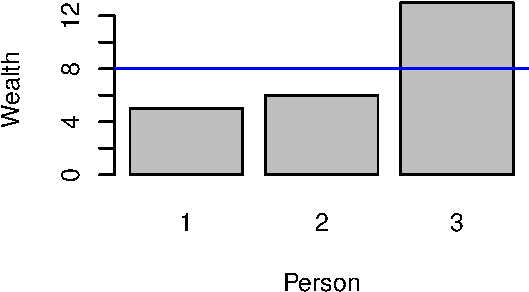
\includegraphics{figure/bar1-1.pdf}
\end{center}

To achieve exact equality, where each person owns 8 units of wealth, person 3
would have to give away 5 units of wealth, 3 units to person 1 and 2 units to
person 2.  That is, $3 + 2 = 5$ units of wealth have to be redistributed, and
5 is about 20.8\% of $5 + 6 + 13 = 24$, the total amount of wealth in the population.  Therefore the Hoover
Index for this population is 20.8\%. 

Note that the amount of wealth that had to be redistributed shows up 
in two ways: 

\begin{itemize}
\item The less wealthy in the population (persons 1 and 2) are $3 + 2 = 5$ units ``short" 
of the mean altogether.
\item The more wealthy in the population (person 3), at 13 units, is $13 - 8 = 5$ units above the mean. 
\end{itemize}

Therefore if we add up the total amount by which each person's wealth differs from the average
wealth (in absolute value) we should get \emph{twice} the amount of wealth that needs 
to be redistributed to achieve complete equality.  To make the following
calculation clearer, let's set $A$ equal to the \emph{amount} of wealth that has
to be redistributed to reach full equality (as opposed to the
\emph{percentage} of total wealth it's necessary to distribute).

Then the first sentence in the above paragraph states: 

$$\sum_{i = 1}^N |x_i - \bar{x}| = 2A$$

If we divide both sides by 2, we get: 

$$\dfrac{\sum_{i = 1}^N |x_i - \bar{x}|}{2} = A$$

which is equivalent to: 

$$A = \dfrac{\sum_{i = 1}^N |x_i - \bar{x}|}{2}$$

Now this is the amount of wealth that needs to be distributed; to get 
the percentage, we divide by the total wealth $\sum_{x = 1}^N x_i$
and multiply by 100\%: 

$$H = \dfrac{\sum_{i = 1}^N |x_i - \bar{x}|}{2\sum_{i = 1}^N x_i} \times 100\%$$

We can use the fact that $\sum_{x = 1}^N x_i = N\times \bar{x}$, which follows 
from $\bar{x} = \sum_{x = 1}^N x_i$ to get this useful alternate form: 

$$H = \dfrac{\sum_{i = 1}^N |x_i - \bar{x}|}{2N\bar{x}}.$$

As a check, let's apply the formula to our simple example.  Recall that 
the wealth values were 5, 6, and 13 units.  

\begin{align*}
H &= \dfrac{\sum_i |x_i - \bar{x}|}{2\sum_i x_i}\times 100\% \\[10pt]
&= \dfrac{|5 - 8| + |6 - 8| + |13 - 8|}{2\times (5 + 6 + 13)} \times 100\% \\[10pt]
&= \dfrac{3 + 2 + 5}{48} \times 100\% \\[10pt]
&= \dfrac{10}{24} \times 100\% \\[10pt]
&= 0.208\bar{3}\times 100\% \\[10pt]
&\approx 20.8\% \\
\end{align*}

\subsection*{Problem 1}  Suppose a population of five people have wealth values
7, 10.5, 12, 12, and 23.  Round your answer to the nearest tenth of a percent.
Find the Hoover Index. (Solution is on page xx) 

\subsection*{Bounds on the Hoover Index}

If everyone in the population has the same amount of wealth, then no wealth
needs to be redistributed to achieve full equality.  Therefore $H$ can equal
0\% in this extreme case.  It can never be negative. 

Now let's consider how large the Hoover Index could be.  First, it's clear that
The Hoover Index cannot exceed 100\%.  The only way to redistribute more than 100\%
is to distribute some of the wealth more than once (i.e., give one person some money, then
later take it back and give it to a second person).
This is unnecessary, because you could gave given the second person the money in 
the first place.

Let's imagine a population of five people where one person owns all the wealth.
To achieve full equality, we have to divide that one person's wealth into five
equal parts, and redistribute four of the five parts.  In other words, 
$4/5 = 80\%$ of the wealth must be distributed.

If the population consisted of 99 people and one person with all the wealth, then 
we would divide that wealth into 100 equal parts and distribute 99 of those parts
to the others who initially had no money.  Therefore $H = 99/100 = 99\%$. 

We could construct larger and larger examples of this type in which the Hoover
Index is arbitrarily close to 100\%.  Therefore we conclude that for any 
population, $$0\% \le H < 100\%.$$

\subsection*{Problem 2}

Suppose everyone in a population has his or her wealth doubled.  Will
that affect the Hoover Index?  What if, instead, each person receives 
\$10{,}000---will the Hoover Index be affected?  Finally, suppose a wealthy person
gives a poorer person a small portion of their wealth (not enough to bring the poorer 
person up to average).  Will $H$ be affected?  You can use a very small
hypothetical population to investigate these questions, for example, three people
with wealth amounts \$1000, \$2000, and \$3000.

\newpage
\section*{The Gini Index}

The Gini Index, named after the statistician Corrado Gini (1884--1965), is 
another, slightly more complex measure of inequality in the distribution of 
goods such as wealth across a population.  We'll derive a formula for the 
Gini Index.

Let's consider a population of five people and hypothetical values 
for the net worth of each.  The numbers will be small (perhaps we'll work in 
units of \$10{,}000) and chosen to make the computations simple. 

\begin{center}
\begin{tabular}{lc}
\toprule
Person & Units of Wealth \\ \midrule
Aya & 10 \\ \midrule
Ben & 19 \\ \midrule 
Carmen & 8 \\ \midrule
Dan & 9 \\ \midrule
Elana & 4 \\ 
\bottomrule
\end{tabular}
\end{center}
 
Just as with the Hoover Index, the goal is to capture the amount of wealth inequality
in the form of a single statistic.  We will start with a simple idea, and gradually refine it until
we have something useful. 

\subsection*{First Attempt}  Suppose we choose a pair of people from our population at 
random and compute the difference in wealth between them.  We would like a
statistic which estimates this difference (on average) as accurately as possible.

That's exactly what the (arithmetic) mean of the absolute value of the differences
in wealth is designed to estimate.  Let's try that.  I'll call this ``AWD1"
for "average wealth difference, attempt 1".

Using summation notation, we will compute: 

$$\text{AWD1} = \dfrac{\displaystyle\sum_{\text{pairs \{i, j\}}} |x_i - x_j|}{\text{number of pairs}}$$

For each pair of people, we'll subtract one wealth amount from the other, take the absolute value,
and finally take the mean of all those absolute values.  

For example, for the pair $\{\text{Aya},\ \text{Ben}\}$, we calculate $|10 - 19| = |-9| = 9$.  

We don't need to include a term $\{\text{Ben},\ \text{Aya}\}$, because that is the same
pair of people.  

$\{\text{Aya},\ \text{Aya}\}$ is not a true ``pair" of people (most likely, it would be
interpreted as a set with a single person as its one element), so we won't consider such things in the mean. 

%How many pairs of people are there altogether?  Here's a diagram which 
%connects each distinct pair of people with a line segment:

%<<k5, fig.height = 4, fig.width = 4, echo=FALSE, message=FALSE, warning=FALSE, crop = TRUE, include = FALSE>>=
%library(igraph)
%igraph.options(vertex.color = "white", vertex.size = 90, weight.scale = 3)
%g <- graph_from_literal("Aya"--"Ben"--"Carmen"--"Dan"--"Elana"--"Aya"--"Carmen"--"Elana"--"Ben"--"Dan"--"Aya")
%plot(g)
%@
%\begin{center}
%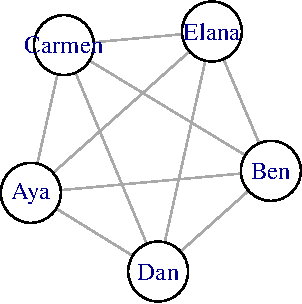
\includegraphics{figure/k5-1.pdf}
%\end{center}

%We can also enumerate them with a table. The bullet points indicate the distinct
%pairs of people; the boxes that are crossed out are either repeats of pairs that 
%were already counted or correspond to ``pairs" of a single person listed twice.  

%\begin{center}
%\begin{tabular}{|l|c|c|c|c|c|}
%\toprule
%     & Aya & Ben & Carmen & Dan & Elana \\ \midrule 
%Aya    & $\times$ & $\bullet$  &  $\bullet$ & $\bullet$ & $\bullet$ \\ \midrule
%Ben    & $\times$  & $\times$  & $\bullet$  & $\bullet$ & $\bullet$   \\ \midrule 
%Carmen & $\times$  &  $\times$    &   $\times$      & $\bullet$ & $\bullet$ \\ \midrule
%Dan    & $\times$  &  $\times$    &   $\times$      &  $\times$    & $\bullet$ \\ \midrule
%Elana  & $\times$   &  $\times$    &  $\times$       &  $\times$    &  $\times$     \\ \bottomrule
%\end{tabular}
%\end{center}

%So, either count the number of lines in the first diagram or the number of bullets
%in the second.  There are ten pairs altogether.  In a population of $n$ people, there will always
%be $\dfrac{n(n - 1)}{2}$ distinct pairs to consider. 

%Here is the calculation of our tentative statistic $awd1$ (average wealth difference)
%for our example: 

I'll do the calculation in tabular form.  First, note that we can systematically
write down all the distinct pairs of people this way: 
\begin{enumerate}
\item First write all the pairs including the first person in our list (Aya).
\item Second, write all the pairs including the second person in our list, Ben,
without repeating the pair $\{\text{Ben}, \text{Aya}\}$.  
\item Third, write all the pairs including the third person, without repeating any pairs.
\item And so forth \ldots 
\end{enumerate}

\begin{center}
\begin{tabular}{l}
\toprule
Aya/Ben \\ \midrule
Aya/Carmen \\ \midrule
Aya/Dan \\ \midrule
Aya/Elana \\ \midrule
Ben/Carmen \\ \midrule
Ben/Dan \\ \midrule
Ben/Elana \\ \midrule
Carmen/Dan \\ \midrule
Carmen/Elana \\ \midrule
Dan/Elana \\ 
\bottomrule
\end{tabular}
\end{center}

Now for each pair, compute the absolute value of the wealth difference, then 
take the mean: 

\begin{center}
\begin{tabular}{lc}
\toprule
Pair         & absolute difference in wealth \\ \midrule
Aya/Ben      & $|10 - 19| = 9$  \\ \midrule
Aya/Carmen   & $|10 - 8|  = 2$  \\ \midrule
Aya/Dan      & $|10 - 9|  = 1$  \\ \midrule
Aya/Elana    & $|10 - 4|  = 6$  \\ \midrule
Ben/Carmen   & $|19 - 8|  = 11$ \\ \midrule
Ben/Dan      & $|19 - 9| = 10$ \\ \midrule
Ben/Elana    & $|19 - 4| = 15$ \\ \midrule
Carmen/Dan   & $|8 - 9|  =  1$  \\ \midrule
Carmen/Elana & $|8 - 4|  =  4$  \\ \midrule
Dan/Elana    & $|9 - 4|  =  5$  \\ \bottomrule
Sum          &     $64$ \\
\end{tabular}
\end{center}

The sum of the absolute differences is 64, so the mean of the absolute differences
is $64/10 = 6.4$.

%Now if you prefer, you can organize you work this way, without a table: 
%
%\begin{align*}
%\text{AWD1} &= \dfrac{|10 - 19| + |10 - 8| + |10 - 9| + |10 - 4| + |19 - 8| + |19 - 9| \
%    + |19 - 4| + |8 - 9| + |8 - 4| + |9 - 4|}{10} \\[10pt]
%    &= \dfrac{|-9| + |2| + |1| + |6| + |11| + |10| + |15| + |-1| + |4| + |5|}{10} \\[10pt]
%    &= \dfrac{9 + 2 + 1 + 6 + 11 + 10 + 15 + 1 + 4 + 5}{10} \\[10pt]
%    &= \dfrac{64}{10} \\[10pt]
%    &= 6.4
%\end{align*}

To sum up, if we choose a pair of people from our population at random (with each 
pair being equally likely to be chosen), then our best guess for the difference in 
their wealth is 6.4 units.  We could then use this statistic on a larger scale to estimate
average wealth difference among citizens of an entire country.  

\subsection*{First Refinement}

One issue with this statistic is that it is scale dependent.  Because different countries
use different units of currency, values of $AWD1$ computed for two different countries are
likely not to be directly comparable.  For example, one US dollar historically has value
roughly 100 Japanese yen. 

We will have a much more useful statistic if we can adjust the formula so that 
a particular value has the same meaning regardless of the what units of wealth are 
being used.  This process is called \emph{normalization}. 

Here's what we'll do:  We'll divide our $AWD1$ by the average value of wealth
across the population (which you can check is 10 in this example).

In this case, our initial value of 6.4 becomes 0.64.  We could call that 
AWD2.  You could check that if we multiply all our hypothetical wealth 
values by 5, for example, that would have no effect on our AWD2 statistic.  

Here is how we could express AWD2 using the sigma notation: 

$$\text{AWD2} = \dfrac{\displaystyle\sum_{\text{pairs \{i, j\}}} |x_i - x_j|}{(\text{number of pairs})\times \bar{x}}$$

\subsection*{Second Refinement}

Can we do better?  Some statistics have the nice property that all the possible
values lie in a finite interval of real numbers.  If that's the case, then it's 
especially convenient if we can arrange that that interval be $[0, 1]$. 

Let's look at some extreme hypothetical values of our statistic AWD2.  

One possible scenario is that everyone has the same amount of wealth, say 10 units: 

\begin{center}
\begin{tabular}{lc}
\toprule
Person & Units of Wealth \\
Aya & 10 \\ \midrule
Ben & 10 \\ \midrule
Carmen & 10 \\ \midrule
Dan & 10 \\ \midrule
Elana & 10 \\ \bottomrule
\end{tabular}
\end{center}

Now if we calculate the sum of the wealth differences, we simply get a sum 
of zeros, which totals to 0.  The average wealth equals 10, and $\dfrac{0}{10} = 0$,
so $\text{AWD2} = 0$ in this case. 

Note that AWD2 can never be negative, because the absolute value of any 
real number is at least zero.  Therefore the values of AWD2 is always 
a nonnegative real number. 

At the other extreme, it seems logical that the greatest average difference
may be achieved if one person has very high wealth and everyone else has 
zero (thus driving the average wealth down). 

\begin{center}
\begin{tabular}{lc}
\toprule
Person & Units of Wealth \\
Aya & 10 \\ \midrule
Ben & 0 \\ \midrule
Carmen & 0 \\ \midrule
Dan & 0 \\ \midrule
Elana & 0 \\ \bottomrule
\end{tabular}
\end{center}

The only pairs with different wealth are $\{\text{Aya},\ \text{Ben}\}$,
$\{\text{Aya},\ \text{Carmen}\}$, $\{\text{Aya},\ \text{Dan}\}$, and 
$\{\text{Aya},\ \text{Elana}\}$.  

The sum of all the wealth differences is thus $10 + 10 + 10 + 10 = 40$, and 
if we divide by the number of pairs (10) times the average, which is $(10 + 0 + 0 + 0 + 0)/5 = 2$,
we find that $\text{AWD2} = \dfrac{40}{10\times 2} = 2$.  

It is in fact true that the largest value that AWD2 can attain is 2, when a single
person has all the wealth and everyone else has zero.  Therefore AWD2 always lies
in the interval $[0, 2]$. 

We could therefore properly normalize this statistic by dividing AWD2 by 2. 
This AWD2 is the actual Gini Index.

To summarize, here is a procedure for calculating the Gini Index for a population:

\begin{enumerate}
\item For each pair in the population, find the absolute value of their
wealth difference.
\item Find the average of these absolute wealth differences.
\item Divide that average by twice the mean wealth in the population.
\end{enumerate}

In sigma notation: 
$$G = \dfrac{\displaystyle\sum_{\text{pairs}\ \{i, j\}} |x_i - x_j|}{2(\text{number of pairs})\bar{x}}$$

\subsection*{Example 4}
Consider a population of five people, A, B, C, D, and E, with
wealth values 1, 4, 1, 3, and 10, respectively.  

Let's compute the Gini Index.  I'll use the tabular format again, writing
out one row per pair: 

\begin{center}
\begin{tabular}{lc}
\toprule
Pair & Absolute Wealth Difference \\ \midrule
A/B & $|1 - 4| = 3$  \\ \midrule
A/C & $|1 - 1| = 0$  \\ \midrule
A/D & $|1 - 3| = 2$ \\ \midrule
A/E & $|1 - 10| = 9$ \\ \midrule
B/C & $|4 - 1| = 3$ \\ \midrule
B/D & $|4 - 3| = 1$ \\ \midrule
B/E & $|4 - 10| = 6$ \\ \midrule
C/D & $|1 - 3| = 2$ \\ \midrule
C/E & $|1 - 10| = 9$ \\ \midrule
D/E & $|3 - 10| = 7$ \\ \bottomrule
Sum & 42
\end{tabular}
\end{center}

Now we divide this sum of 42 by $2(\text{number of pairs})\bar{x}$.  The 
number of pairs is once again 10, and the mean of the wealth values is 
$(1 + 4 + 1 + 3 + 10)/5 = 3.8$. 

Therefore: 

\begin{align*}
G &= \dfrac{\sum_{\text{pairs}\ \{i, j\}}|x_i - x_j|}{2(\text{number of pairs})\bar{x}} \\[10pt]
&= \dfrac{42}{2(10)3.8} \\[10pt]
&= 0.55
\end{align*}

\subsection*{Interpreting the Gini Index}

As with the Hoover Index, the Gini Index lies between 0 and 1.  A Gini Index
of 0 means that everyone has the same amount of wealth.  A Gini Index of 1
means a single person has all the wealth and the rest have zero.  The Gini
Indices of countries lie mostly in the range 0.25 to 0.60.  

\subsection*{Comparing the Hoover and Gini Indices}

We have now discussed two measures of the inequality of wealth in a population.  This 
raises the question of how the two measures compare to each other.  We would hope that they
both measure inequality well.  If their values are always equal, that would be interesting 
mathematically, but it would indicate that one is redundant.  

Can one index always be calculated exactly from the other index?  It turns out the answer
to this question is ``no". 

Consider two populations, A and B.  Population A consists of two people, with wealth values 1 and 2 respectively.

Population B consists of three people with wealth values 1, 1, and 2. 

Population A has Hoover Index 16.7\% and Gini Index 33.3\% (to one decimal place). 

Population B has Hoover Index 16.7\% and Gini Index 25\%.

Therefore just knowing the Hoover Index of a population does not imply that we know 
the Gini Index of that population. 

However, the two indices are strongly related, and, for example, a high Gini Index implies 
a high Hoover Index.  Edward Allen has determined a formula\footnote{Edward Allen, ''Relation 
    Between Two Income Inequality Measures: The Gini coefficient and the Robin Hood Index," WSEAS
Transactions on Business and Economics, vol. 19, pp. 760--770, 2022} for the Hoover Index in 
terms of the Gini Index which is accurate to 5\% provided $0 \le G \le 0.95$.  Here is 
that formula: 

\begin{equation*}
    H(G) = 
    \left\{
	\begin{array}{lr}
	    0.74G & \text{if } G \le 0.5 \\
	    0.37 + 0.90(G - 0.50) & \text{if } 0.5 \le G \le 0.8 \\
	    0.64 + 1.26(G - 0.80) & \text{if } 0.8 \le G \le 0.95 \\
	\end{array}
    \right\}
\end{equation*}

The blue graph gives Allen's estimate of the Hoover Index from the Gini Index.
According to this estimate, the Gini Index tends to be slightly larger than the 
Hoover Index for $0 \le G \le 0.95$.

\begin{knitrout}
\definecolor{shadecolor}{rgb}{0.969, 0.969, 0.969}\color{fgcolor}
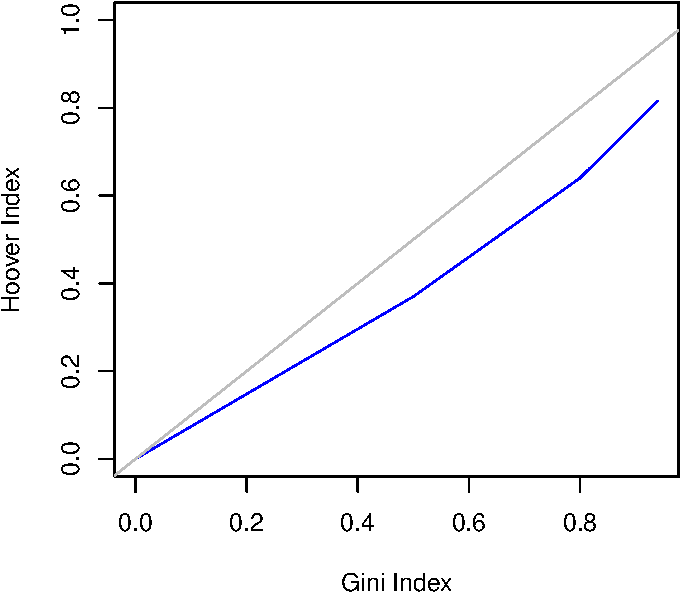
\includegraphics[width=\maxwidth]{figure/unnamed-chunk-1-1} 
\end{knitrout}

\subsection*{An Alternate Formula for $G$}

There is one awkward aspect of the expression for the Gini Index which we have
derived:  It involves a sum over all wealth differences between \emph{pairs}
in the population.  This makes sense conceptually, as we are interested in 
how far apart in wealth different members of the population are.  However, it
raises the issue of how, if we want to compute the Gini Index for a large population,
we are going to enumerate all these pairs.

A more commonly seen formula for $G$ sidesteps this issue at the cost of some
redundancy. To illustrate, let's look back to a previous example, where 
we had to form all distinct pairs using the group Aya, Ben, Carmen, Dan, and Elana.

The following table shows the distinct pairs we formed: 

\begin{center}
\begin{tabular}{|l|c|c|c|c|c|}
\toprule
     & Aya & Ben & Carmen & Dan & Elana \\ \midrule 
Aya    & $\times$ & $\bullet$  &  $\bullet$ & $\bullet$ & $\bullet$ \\ \midrule
Ben    & $\times$  & $\times$  & $\bullet$  & $\bullet$ & $\bullet$   \\ \midrule 
Carmen & $\times$  &  $\times$    &   $\times$      & $\bullet$ & $\bullet$ \\ \midrule
Dan    & $\times$  &  $\times$    &   $\times$      &  $\times$    & $\bullet$ \\ \midrule
Elana  & $\times$   &  $\times$    &  $\times$       &  $\times$    &  $\times$     \\ \bottomrule
\end{tabular}
\end{center}

The bullets indicate the genuinely distinct pairs of two different people.  
The $\times$'s indicate pairs that either were already counted or really
consisted of a single person.  There were ten pairs/bullets.  The Gini
Index is the sum of the 10 absolute wealth differences divide by 
$2\times(\text{number of pairs})\bar{x}$.  

Now if we dispense with this step of enumerating only the ``genuine" pairs 
of two distinct people, include the ``pairs" corresponding to boxes with 
$\times$ symbols in them, it turns out that we will just get \emph{twice}
the sum $\displaystyle\sum_{\text{pairs}\ \{i, j\}} |x_i - x_j|$. 

That's because in the the diagonal corresponding to the ``pairs" $\{\text{Aya}, \text{Aya}\}$,
$\{\text{Ben}, \text{Ben}\}$, \ldots, $\{\text{Elana}, \text{Elana}\}$, all the 
wealth differences are zero.

The pairs below this diagonal are duplicates of the pairs above the diagonal; the people
are just listed in reverse order.  

Therefore we could simply add up the absolute wealth differences over the entire grid,
as indicated below, then divide the sum by 2 to compensate for the double-counting. 

\begin{center}
\begin{tabular}{|l|c|c|c|c|c|}
\toprule
     & Aya & Ben & Carmen & Dan & Elana \\ \midrule 
Aya    & $\bullet$ & $\bullet$  &  $\bullet$ & $\bullet$ & $\bullet$ \\ \midrule
Ben    & $\bullet$ & $\bullet$  &  $\bullet$ & $\bullet$ & $\bullet$   \\ \midrule 
Carmen & $\bullet$ & $\bullet$  &  $\bullet$ & $\bullet$ & $\bullet$ \\ \midrule
Dan    & $\bullet$ & $\bullet$  &  $\bullet$ & $\bullet$ & $\bullet$ \\ \midrule
Elana  & $\bullet$ & $\bullet$  &  $\bullet$ & $\bullet$ & $\bullet$     \\ \bottomrule
\end{tabular}
\end{center}

If we use $x_1$, $x_2$, $x_3$, $x_4$, and $x_5$ to represent the wealth values
for Aya, Ben, Carmen, Dan, and Elana, then this new sum of absolute wealth
differences could be represented by: 
$$\sum_{1\ \le\ i,\ j\ \le\ 5} |x_i - x_j|$$
This just means we add up all the $|x_i - x_j|$ for all possible 
combinations of $i$ and $j$ where $i$ and $j$ are between 1 and 5.  
Note that there are no other restrictions:  $i = 1$ and $j = 1$ are 
included, as are $i = 1$, $j = 2$ and $i = 2$, $j = 1$.  There are 
thus $5\times 5 = 25$ different absolute differences to add up. 

We now have the following formula for the Gini Index, which is equivalent
to the first: 

\begin{align*}
G &= \dfrac{\displaystyle\sum_{\text{pairs}\ \{i,\ j\}} |x_i - x_j|}{2(\text{number of pairs})\bar{x}} \\[10pt]
  &= \dfrac{\displaystyle\sum_{1\ \le i,\ j\ \le n} |x_i - x_j|}{4(\text{number of pairs})\bar{x}} \\
\end{align*}

Now the denominator still refers to the number of pairs of people.  Here we'll use a
useful counting formula:  Given $n$ people, the number of distinct pairs (unordered)
of those people is $\frac{n(n - 1)}{2}$.  We can therefore substitute this into the 
denominator and simplify a bit more: 

\begin{align*}
G &= \dfrac{\displaystyle \sum_{1\ \le i,\ j\ \le n} |x_i - x_j | }{ 4(\text{number of pairs})\bar{x}} \\[12pt]
  &= \dfrac{\displaystyle \sum_{1\ \le i,\ j\ \le n} |x_i - x_j | }{ 4(\frac{n(n - 1)}{2} )\bar{x} } \\[12pt]
  &= \dfrac{\displaystyle \sum_{1\ \le i,\ j\ \le n} |x_i - x_j | }{ 2n(n - 1)\bar{x} } \\
\end{align*}

[This is clearly far too notation-heavy for Math 106; perhaps the formula could be
described verbally.]

[Question: Does this have $n(n - 1)$ in the denominator instead of $n^2$ in order for it to
be an unbiased estimator for $G$?  This formula with $n(n - 1)$ seems to agree with the
Gini function in DescTools.]

\newpage
\section*{The Lorenz Curve}
\bigskip

Based in Switzerland, Credit Suisse is a large investment bank and financial 
services company which was founded in 1856.  Credit Suisse one of several institutions
considered by the Swiss National Bank to be a ``systemically important bank" in that
its failure could have a severe impact on the world economy.  Regulators require
systemically important banks to meet stricter standards than other banks to
prevent failure.  It is therefore in the interest of Credit Suisse to have a
clear understanding of the global economy.  After the ``Great Recession"
of the late 2000's, Credit Suisse began publishing annual Global Wealth Reports
and Databooks.   The following chart appeared in the 2016 Global Wealth Report:

\begin{center}
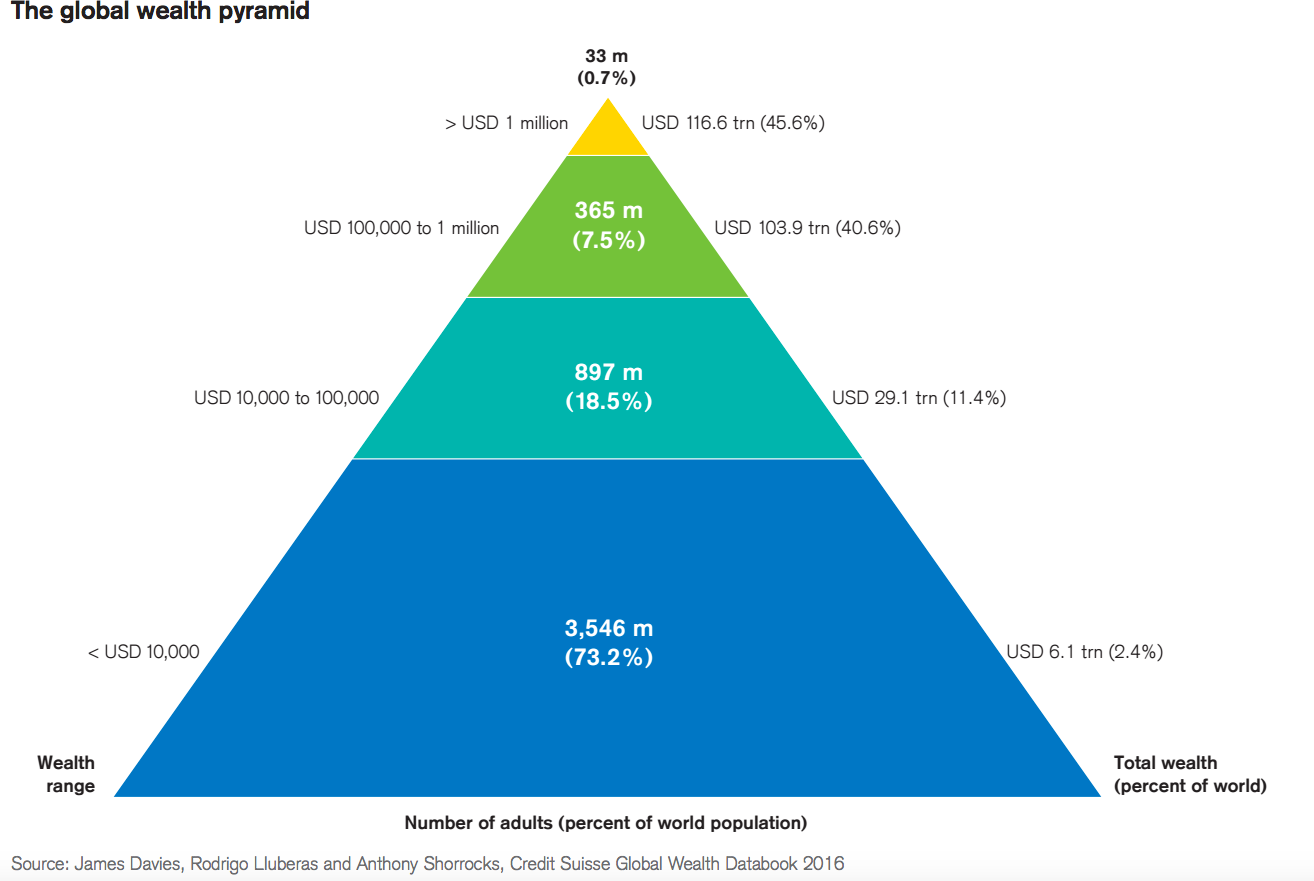
\includegraphics[width = 11cm]{graphs/globalwealthpyramid2016.png}
\end{center}
(Image source:  {\scriptsize \url{https://www.statista.com/chart/11857/the-global-pyramid-of-wealth/}, 
accessed 12/19/2022})

This chart conveys information about how wealth is distributed worldwide.
In particular, it describes what percentage of adults have wealth within
various ranges.  For example, according to the numbers along the left side and the 
middle of the triangle, 73.2\% of adults worldwide have wealth less than 
US\$10{,}000 as of 2016.  About 0.7\% of 
adults have wealth greater than \$1 million.  

The numbers on the right side tell us, for example, that the bottom 73.2\%
of the adult population (in terms of wealth) own 2.4\% of the world's 
wealth, while the top 0.7\% of adults own 45.6\% of the world's wealth. 

While this chart provides a vivid display of quite a bit of information, it does
raise some questions about how we could analyze wealth distributions more deeply.
For example:

\begin{enumerate}
\item The areas of the four colored regions correspond to the percentage
of adults in a particular wealth range.  For example, the area of the blue region
is about 73.2\% of the area of the entire triangle.  The area of the yellow peak
is about 0.7\% of the area of the triangle.  Clearly the yellow area is much smaller
than the blue area, but by how much?  That is difficult to judge.  People have 
difficulty making accurate comparisons of two areas; they tend to do better
when comparing lengths to one another.  The blue area
at the bottom is over 100 times as large as the yellow area at the top---is
that about what you would have guessed without being given their areas?
Perhaps there are better ways to communicate the same information? 

\item The wealth ranges (0 to \$10{,}000, \$10{,}000--\$100{,}000, etc.) are 
somewhat arbitrary, and based on US dollars.  Perhaps this chart should be 
called ``\emph{A} Global Wealth Pyramid" rather than ``\emph{The} Global Wealth
Pyramid".  

\item What if we wanted to make similar charts for individual countries
which don't use US dollars?  Is there a step-by-step procedure we could use
which doesn't depend on the unit of currency? 
\end{enumerate}

\subsection*{Defining the Lorenz Curve}
\bigskip
Let's go back to the Global Wealth Pyramid:

\begin{center}
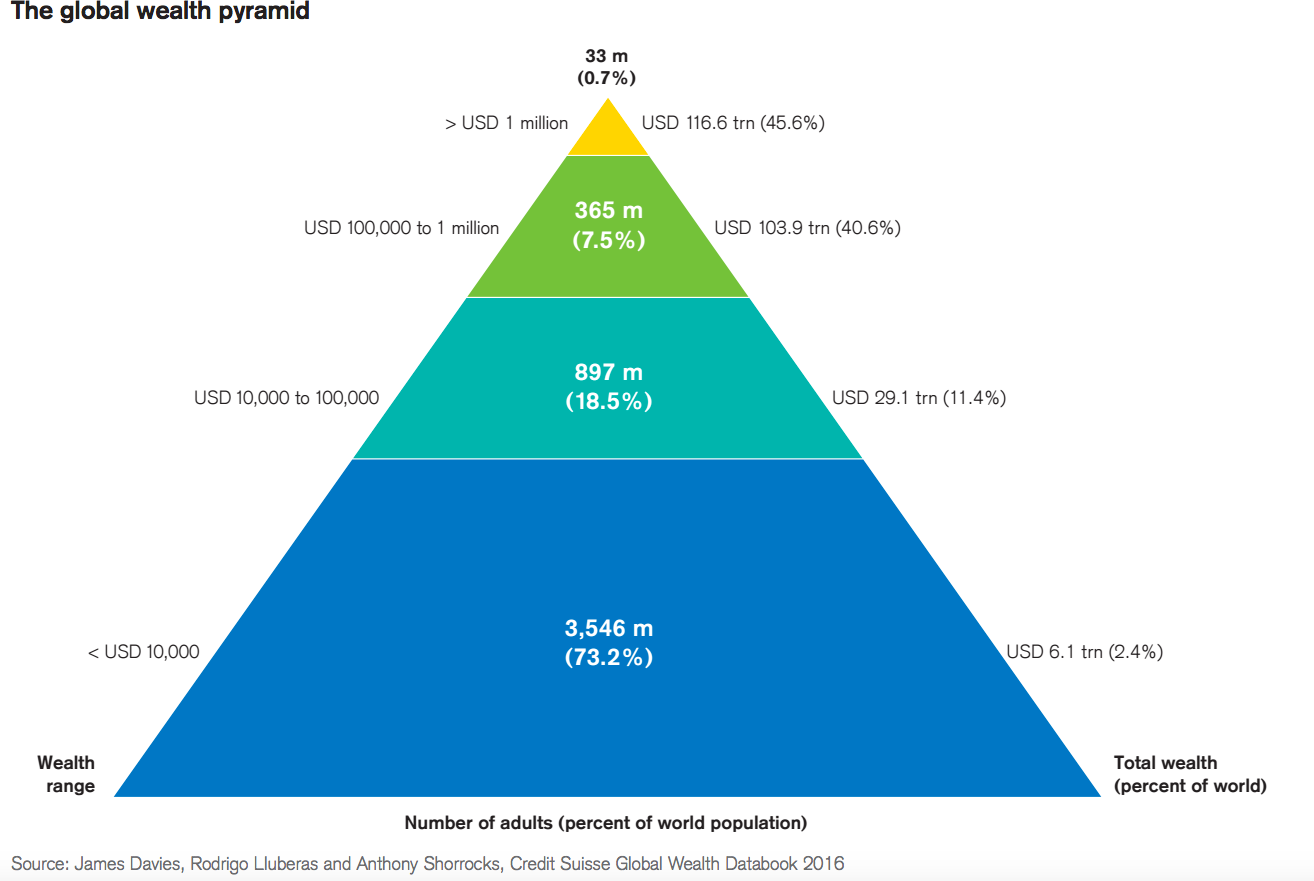
\includegraphics[width = 12cm]{graphs/globalwealthpyramid2016.png}
\end{center}

We'll extract the percentages and put them in a table: 
\begin{center}
\begin{tabular}{ccc}
\toprule
Group & Percentage of Population & Percentage of Wealth \\ \midrule
1     & 73.2                     &  2.4 \\ \midrule
2     & 18.5                     & 11.4 \\ \midrule
3     &  7.5                     & 40.6 \\ \midrule 
4     &  0.7                     & 45.6 \\ \bottomrule
\end{tabular}
\end{center}
The American economist Max Lorenz (1876--1959) devised a way to transform this 
table into a more useful format by creating ``cumulative" versions of the
percentages of population and wealth at each level.  The Lorenz Curve gives a 
very detailed description of the distribution of wealth in a population.  In fact,
both the Hoover and Gini indices, as well as other measures of wealth inequality
can be derived from it.

Here's a description of the idea in words: 

From row 1:  The bottom 73.2\% of the population owns 2.4\% of the wealth.

From row 2:  The bottom $73.2\% + 18.5\% = 91.7\%$ of the population owns $2.4\% + 11.4\% = 13.8\%$
of the wealth.


From row 3:  The bottom $73.2\% + 18.5\% + 7.5\% = 99.2\%$ of the population owns
$2.4\% + 11.4\% + 40.6\% = 54.4\%$ of the wealth.

The fourth row essentially says the bottom 99.9\% of the population owns 100\% of 
the wealth (the first percentage should in theory be 100\% rather than 99.9\%; the discrepancy is due 
to rounding error).  We could even add a zeroth row, which states that the bottom 0\% of the population owns
0\% of the wealth, which will give us one additional row.  Notice we don't need 
a column for Group number anymore:
\begin{center}
\begin{tabular}{ccccc}
\toprule
The bottom\, & \rule{1cm}{0.4pt} & \%  \,  Own\, & \rule{1cm}{0.4pt}\% & \, of the wealth \\ \midrule
& 0 &    & 0 & \\ \midrule
& 73.2 & & 2.4 & \\ \midrule
& 91.7 & & 13.8 & \\ \midrule
& 99.2 & & 54.4 & \\ \midrule
& 100 &  & 100 & \\ \bottomrule
\end{tabular}
\end{center}
We could now think of each row as representing an ordered pair, and plot
the resulting points.  The points are:

$$(0, 0),\ (73.2, 2.4),\ (91.7, 13.8),\ (99.2, 54.4),\ (100, 100)$$


\begin{center}
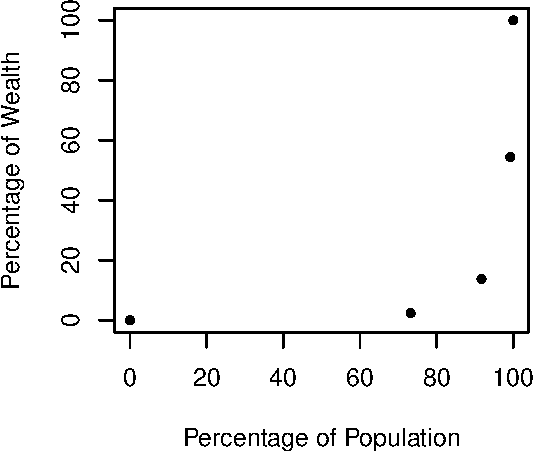
\includegraphics{figure/plota-1.pdf}
\end{center}

\subsection*{The Lorenz Curve for Canada}

Next, we'll look at some data from a different population---the residents of Canada.
We'll use statistics drawn from the World Bank's Poverty and Equity database 
({\scriptsize \url{datacatalog.worldbank.org/search/dataset/0038020/Poverty-and-Equity-Database}})

Let's separate the population of Canada into two groups:  The median (individual)
net worth is that value such that 50\% of individuals in Canada have net worth 
less than that amount, and 50\% have more than that amount. 

The median value divides the population into two halves, a wealthier half, and 
the poorer half. 

According to the database, the poorer half of the population of Canada owns
about 28.2\% of the total wealth (so the wealthier half owns about 100\% minus
28.2\% or 71.8\% of the wealth.)  The poorer half of the population has than 
half the wealth because they're poorer, of course!  The fact that their share
of the wealth is only 28.2\% rather than 50\% indicates there is \emph{some}
wealth inequality in Canada.

In fact, this gives us one point on the graph of the Lorenz Curve for Canada.  
Let's call the function $L$.  We have found that: 
$$L(0.50) = 0.282.$$
Equivalently, the point $(0.50, 0.282)$ lies on the graph of $L$. 

By dividing up the population of Canada into more groups (by wealth), we can find
more points on the Lorenz Curve.  Here are some further statistics from the World
Bank database (2016 and 2017 numbers):
\begin{quote}
The bottom 20\% own 7.1\% 

The bottom 40\% own 19.5\%

The bottom 60\% own 37.0\%

The bottom 80\% own 59.9\%
\end{quote}
We also know that the bottom 100\% (which is the entire population of Canada) owns
100\% = 1.00 = 1 of the wealth, and the bottom 0\% own 0\% of the wealth
(assuming no negative wealth here). This gives us six points on the graph of $L$, plotted below: 

\begin{center}
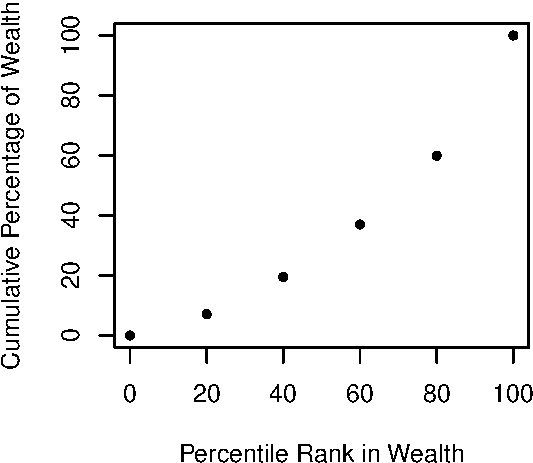
\includegraphics{figure/Lorenz1-1.pdf}
\end{center}
I've labeled the horizontal axis using the term ``percentile".  The 20th 
percentile in wealth is that wealth value $x$ such that 20\% of the population
owns less than $x$ dollars in wealth. 

With more and more data, we can fill in the graph of $L$ so that it approximates
a continuous, unbroken curve.  In principle, this process of filling in more points
cannot go on forever, because the population of Canada is finite---there are a bit 
fewer than 40 million residents currently, which means even if we had complete wealth 
information on every citizen, there could not be more than 40 million points on the
graph!  However, it's far easier to work with a function defined by a continuous curve than
a graph with 40 million points.  

In fact, it's likely that with just the six points plotted above, if we draw a
continuous curve through them the result will be close enough to the ``true" graph
of $L$ to be useful.  


\begin{center}
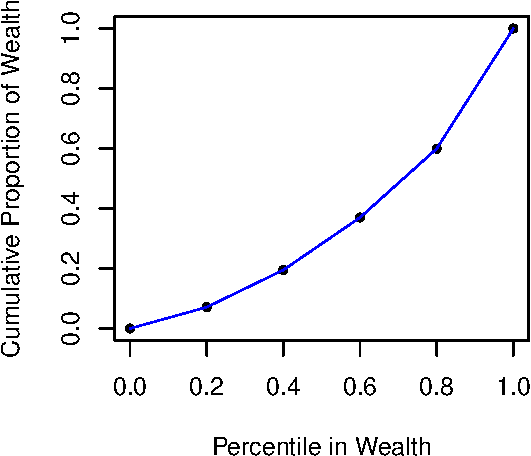
\includegraphics{figure/Lorenz2-1.pdf}
\end{center}

\subsection{The Lorenz Curve from Scratch}

Let's consider a hypothetical population of eight people: 
\medskip
\begin{center}
\begin{tabular}{lc}
\toprule
Name & Wealth \\ \midrule
Nicole & 11 \\ \midrule
Deshawn & 14 \\ \midrule
Reid    & 7 \\ \midrule
Saniya  & 11 \\ \midrule
Evan    & 5 \\ \midrule
Ari     & 10 \\ \midrule
April   & 3 \\ \midrule
Cameron & 19 \\ \bottomrule
\end{tabular}
\end{center}
\medskip

The next steps will be much easier if we sort the table by wealth; I'll rewrite
the rows so that the wealth values are in descending order.  I'll also add 
a Totals row at the bottom.
\medskip

\begin{center}
\begin{tabular}{lc}
\toprule
Name & Wealth \\ \midrule
Cameron & 19 \\ \midrule
Deshawn & 14 \\ \midrule
Saniya  & 11 \\ \midrule
Nicole  & 11 \\ \midrule
Ari     & 10 \\ \midrule
Reid    & 7  \\ \midrule
Evan    & 5  \\ \midrule
April   & 3  \\ \bottomrule
Totals  & 80
\end{tabular}
\end{center}
\medskip

For the next step, we want to divide the sorted table into a number of (approximately)
equally sized groups.  The more groups, the more points on the Lorenz Curve we'll get.  
We only have eight in our population, so I'll chose to divide them into four groups
of two people.  

\begin{center}
\begin{tabular}{lc}
\toprule
Name & Wealth \\ \midrule
\rowcolor{gray!50}
Cameron & 19 \\ \midrule
\rowcolor{gray!50}
Deshawn & 14 \\ \midrule
Saniya  & 11 \\ \midrule
Nicole  & 11 \\ \midrule
\rowcolor{gray!50}
Ari     & 10 \\ \midrule
\rowcolor{gray!50}
Reid    & 7  \\ \midrule
Evan    & 5  \\ \midrule
April   & 3  \\ \bottomrule 
Totals  & 80 \\
\end{tabular}
\end{center}

Cameron and Deshawn make up the wealthiest group.  It contains two out of the population
of eight people, so this group consists of the top 25\% in terms of wealth. 

The next wealthiest 25\% consists of Saniya and Nicole.  Then comes the group of 
Reid and Ari, and finally, Evan and April make up the bottom 25\%.  

Now let's pool the total wealth within each of the four groups.  For example,
the total wealth of the top group is $19 + 14 = 33$ units of wealth.  Here
are the results: 

\begin{center}
\begin{tabular}{lcc}
\toprule
Name & Wealth & Group Wealth \\ \midrule
\rowcolor{gray!50}
Cameron & 19 & \\ \midrule
\rowcolor{gray!50}
Deshawn & 14 & 33 \\ \midrule
Saniya  & 11 &    \\ \midrule
Nicole  & 11 & 22 \\ \midrule
\rowcolor{gray!50}
Ari     & 10 &    \\ \midrule
\rowcolor{gray!50}
Reid    & 7 & 17  \\ \midrule
Evan    & 5  &    \\ \midrule
April   & 3  & 8  \\ \midrule
Totals  & 80  & 80 \\ \bottomrule
\end{tabular}
\end{center}

The Lorenz Curve is a ``cumulative" function, so we'll add a new cumulative 
column.  It gives the total wealth of a group plus the wealth of every group 
below it.

\begin{center}
\begin{tabular}{lccc}
\toprule
Name & Wealth & Group Wealth & Cumulative Group Wealth \\ \midrule
\rowcolor{gray!50}
Cameron & 19 &  & \\ \midrule
\rowcolor{gray!50}
Deshawn & 14 & 33 & 80 \\ \midrule
Saniya  & 11 &    \\ \midrule
Nicole  & 11 & 22 & 47 \\ \midrule
\rowcolor{gray!50}
Ari     & 10 &  &  \\ \midrule
\rowcolor{gray!50}
Reid    & 7 & 17 & 25 \\ \midrule
Evan    & 5  &  &  \\ \midrule
April   & 3  & 8 & 8  \\ \midrule
Totals  & 80  & 80  &\\ \bottomrule
\end{tabular}
\end{center}

Finally, we convert the Cumulative Group Wealth to percentages by 
dividing the Cumulative Group Wealth Column numbers by 80 (the total wealth),
then multiplying by 100\% (and rounding a bit if necessary):

\begin{center}
\begin{tabular}{lcccc}
\toprule
Name & Wealth & Group Wealth & \makecell{Cumulative \\ Group Wealth} & \makecell{Cumulative \\ Group Wealth (\%)} \\ \midrule
\rowcolor{gray!50}
Cameron & 19 &  &  & \\ \midrule
\rowcolor{gray!50}
Deshawn & 14 & 33 & 80 & 100\% \\ \midrule
Saniya  & 11 &  &  & \\ \midrule
Nicole  & 11 & 22 & 47 & 58.75\% \\ \midrule
\rowcolor{gray!50}
Ari     & 10 &  &  & \\ \midrule
\rowcolor{gray!50}
Reid    & 7 & 17 & 25 & 31.25\% \\ \midrule
Evan    & 5  &  &  & \\ \midrule
April   & 3  & 8 & 8 & 10\% \\ \midrule
Totals  & 80  & 80  & & \\ \bottomrule
\end{tabular}
\end{center}

This table now gives us four values of the Lorenz Curve Function.  It 
says that the bottom $25\%$ (or 0.25 in decimal form) own $10\%$ of the
wealth, the bottom $25\% + 25\% = 50\%$ (or 0.50) own 31.25\% of the 
wealth, the bottom 75\% (or 0.75) own 58.75\% of the wealth, and the bottom 100\% 
own 100\% of the wealth.  This last statement is always true of course; similarly,
the bottom 0\% own 0\% of the wealth.  Here's a summary, with all values rounded 
to two decimal places: 

\begin{center}
\begin{tabular}{rr}
\toprule
$x$ & $y$ \\ \midrule
0.00   & 0.00 \\ \midrule
0.25 & 0.10 \\ \midrule
0.50 & 0.31 \\ \midrule
0.75 & 0.59 \\ \midrule
1.00 & 1.00 \\ \bottomrule
\end{tabular}
\end{center}

Here's a plot of those five points:

\begin{center}
\begin{knitrout}
\definecolor{shadecolor}{rgb}{0.969, 0.969, 0.969}\color{fgcolor}
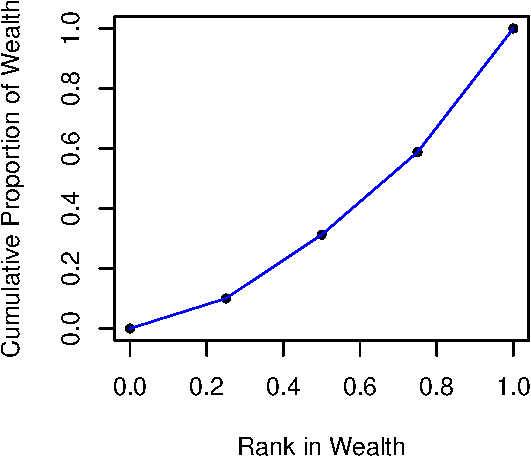
\includegraphics[width=\maxwidth]{figure/Lorenz0-1} 
\end{knitrout}
\end{center}

Note that both the horizontal and vertical coordinates always lie between 0 and 1.
This makes it easy to compare Lorenz curves between multiple countries at a 
glance.  

\newpage

\section*{Solutions to Problems}
\bigskip

\subsection*{Problem 1} 
Suppose a population of five people have wealth values
7, 10.5, 12, 12, and 23.  Round your answer to the nearest tenth of a percent.
Find the Hoover Index. 

\textbf{Solution:}

We use the notation $x_1 = 7$, $x_2 = 10.5$, $x_3 = 12$, $x_4 = 12$, and $x_5 = 23$.

The average of these wealth amounts is: 

$$\bar{x} = \dfrac{7 + 10.5 + 12 + 12 + 23}{5} = = 12.9$$

Then:
\begin{align*} 
H &= \dfrac{\sum_{i = 1}^5}{2\sum_{x = 1}^5 x_i} \times 100\% \\[10pt]
&= \dfrac{ |7 - 12.9| + |10.5 - 12.9| + |12 - 12.9| + |12 - 12.9| + |23 - 12.9|}{2\times 5\times 12.9} \times 100\% \\[10pt]
&= \dfrac{5.9 + 2.4 + 0.9 + 0.9 + 10.1}{129} \times 100\% \\[10pt]
&= 0.1566 \times 100\% \\[10pt]
&= 15.7\%
\end{align*}

\subsection*{Problem 2}
Suppose everyone in a population has his or her wealth doubled.  Will
that affect the Hoover Index?  What if, instead, each person receives 
\$10{,}000---will the Hoover Index be affected?  Finally, suppose a wealthy person
gives a poorer person a small portion of their wealth (not enough to bring the poorer 
person up to average).  Will $H$ be affected?  You can use a very small
hypothetical population to investigate these questions, for example, three people
with wealth amounts \$1000, \$2000, and \$3000.

\textbf{Answers:}  No, yes (unless they all were equally wealthy at the beginning), yes.
These are three properties that ``good" measures of inequality should have.

\theendnotes


\end{document}
\end
